\chapter{Introduction}

The internet, as we know it today, heavily relies on the use of the HTTP protocol. Not only is it
used by web browsers to interact with websites, it also serves as a transport medium for REST web
APIs or popular technologies such as gRPC and GraphQL\@.

Currently, the latest version of the protocol is HTTP/2 published in 2015~\cite{rfc7540}. HTTP/2
improved on its predecessor HTTP/1.1~\cite{rfc7230} by introducing features such as request
multiplexing over a single TCP connection, header compression and the server-push feature, allowing
it to significantly reduce loading times of web pages and generally improve the efficiency of the
web~\cite{deSaxce2015}.

However, some performance aspects of the HTTP/2 protocol cannot be improved by adding more features
or otherwise changing the application layer of the HTTP protocol stack, because the problems are
caused by behavior of the transport protocols used underneath.
\todo{add reference to the analysis? Who has found out where is the bottleneck of HTTP/2?}

Combination of request multiplexing in HTTP/2 and TCP's guaranteed in-order packet delivery leads to
a situation where the loss of a TCP packet bearing data for one request will delay transmission of
packets bearing data for other requests. This problem is generally known as \textit{head-of-line
blocking}\footnote{More detailed description of head-of-line blocking can be found e.g\@. at \url{https://en.wikipedia.org/wiki/Head-of-line_blocking}.}.

Another area where HTTP/2 protocol can be improved is the HTTPS connection establishment latency.
HTTPS~\cite{rfc2818} is an extension to the HTTP protocol, which makes the connection encrypted by
inserting TLS protocol layer between HTTP and TCP layer. Establishing HTTPS connection requires
first establishing TCP connection --- performing the three-way handshake --- and then performing
another handshake for TLS layer. Figure~\ref{fig:https-packets} illustrates the sequence of packets that has to be sent before the first HTTP request packet.

\begin{figure}[h]
  \centering
  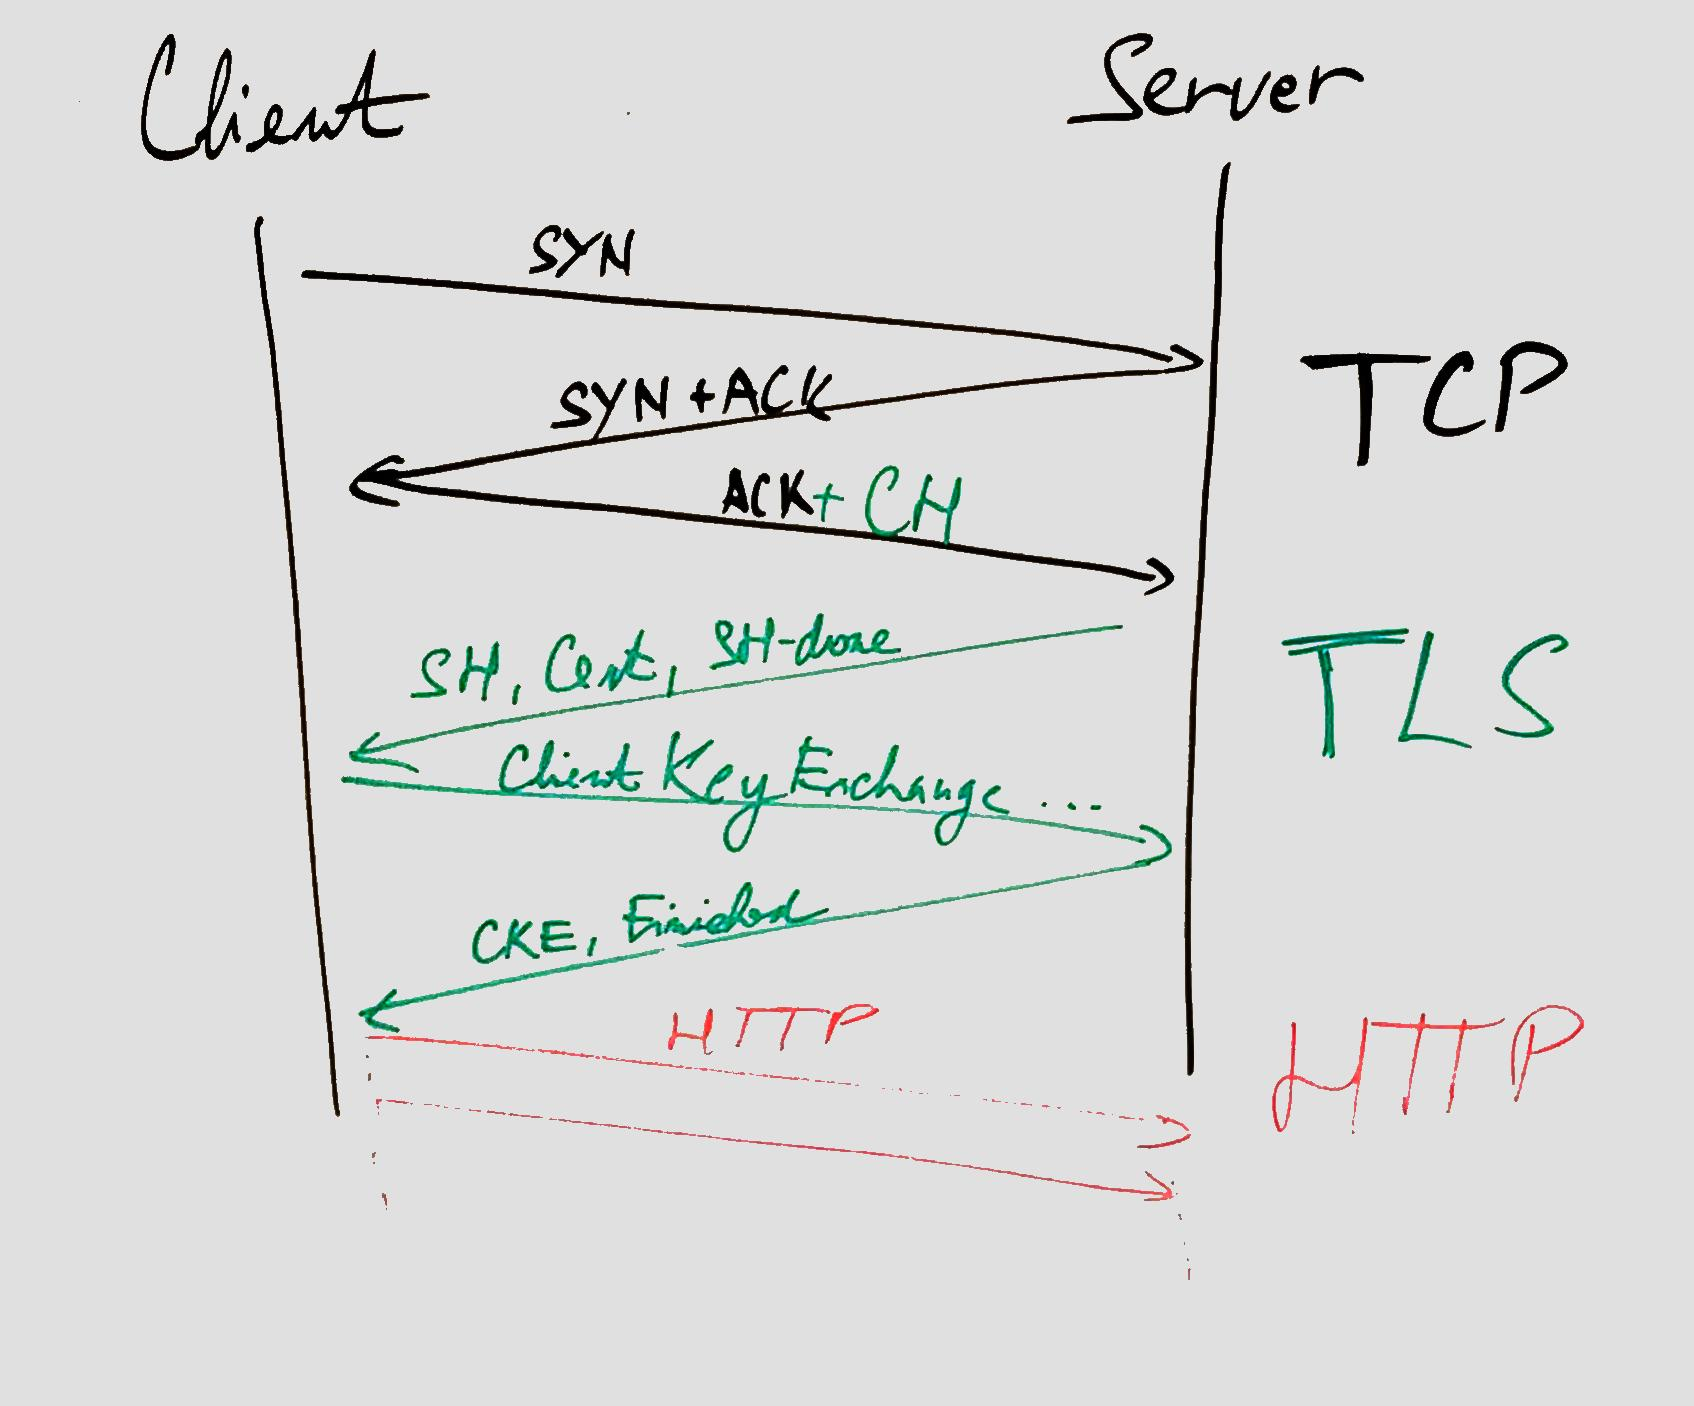
\includegraphics[width=0.6\textwidth]{img/01-https-connection-packets}
  \caption{Simplified view of the packets sent during HTTPS connection establishment}\label{fig:https-packets}
\end{figure}

More and more websites enforce the use of HTTPS to protect the privacy of their users. In August
2020, 96 out of top 100 viewed websites actively redirect to HTTPS, and more than 75\% of all
network traffic from Chrome web browser used HTTPS~\cite{googleTransparency}. With HTTPS becoming the
norm, almost all connections suffer from the increased latency incurred by the additional TLS handshake.

The next version of the HTTP protocol --- HTTP/3~\cite{draft-ietf-quic-http-29} --- addresses these
problems by replacing the TCP and TLS layer with brand new UDP-based protocol named
QUIC\footnote{Originally intended as the acronym for Quick UDP Internet Connection, but during
standartization QUIC has been changed to be the actual name of the protocol.}, and shifting
multiplexing capability from application to transport layer. The relationships between protocols on
HTTP/2 and HTTP/3 stacks are illustrated in figure~\ref{fig:http2-vs-http3-stack}.

\begin{figure}[h]
  \centering
  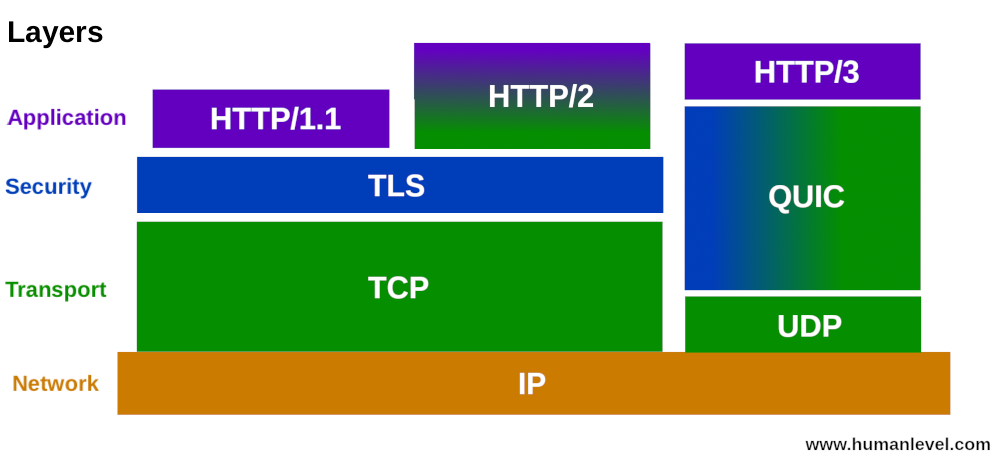
\includegraphics[width=\textwidth]{img/01-pile-http-protocol}
  \todo{Redraw this without HTTP/1.1 in inkscape, indicate which parts of the stack implement stream
    multiplexing, encryption, reliability etc.}
  \caption{Comparison between HTTP/2 and HTTP/3 protocol stacks}\label{fig:http2-vs-http3-stack}
\end{figure}

\todo{possibly more comments on the figure will go here}

Although QUIC development is tied with that of HTTP/3, it is designed as a general-purpose transport
layer protocol that can be used for other application level protocols as well. The main improvements
of QUIC over TCP+TLS can be summarized in following points:

\begin{itemize}
  \litem{Stream multiplexing}
    QUIC provides abstraction of multiple streams multiplexed on a single connection at the
    transport level. And because loss detection and retransmission is implemented also at the QUIC
    layer, rather than UDP, the protocol does not exhibit the \textit{head-of-line blocking}
    problem described above.

  \litem{Faster connection establishment} QUIC still performs TLS 1.3 handshake, but it does so in
    parallel with TCP-like three-way-handshake for the base protocol. This combined handshake
    requires fewer round-trips and therefore reduces latency. QUIC also supports TLS 1.3 Zero Round
    Trip Time Resumption (0-RTT for short). The 0-RTT mode of operation allows a client to cache
    some session information allowing it to send application data with the very first packet in
    future connection to the same server. This effectively reduces the latency by another round
    trip, but makes such requests vulnerable to repeat attacks. More detailed description of 0-RTT
    can be found online, e.g\@. on Cloudflare's blog~\cite{cloudflare-0rtt}.

  \litem{Always encrypted} TLS handshake is a mandatory part of connection establishment and
    therefore QUIC connections are always encrypted. This makes QUIC secure-by-default and no extra
    steps need to be taken by the application protocol to achieve security.

  \litem{Separating connection identity from peer's IP address} QUIC protocol does not use peers
    IP addresses to identify connections, but instead uses connection IDs which are 8 to 20 byte
    sequences negotiated during connection establishment. This makes QUIC very attractive for
    mobile devices, which can switch between multiple IP addresses. This happens e.g\@. when device
    switches from Wi-Fi to cellular data network. Ordinarily, the existing connection has to be terminated and new connection established from the new IP address. QUIC, on the other hand, can migrate the connections in a way that is transparent to the application layer.

    This feature also enables QUIC extensions like Multipath
    QUIC~\cite{draft-deconinck-quic-multipath-04}, which allows simulataneous use of multiple
    network interfaces for a single connection to achieve greater throughput.

\end{itemize}

As of August 2020, the specifications of HTTP/3 and QUIC are still at draft stage, but the
standartization process is believed to be very close to complete. There are already multiple
implementations of the draft versions of the standard and many of these implementations are backed
by big companies such as Cloudflare, Facebook and Microsoft.

Experiments with these implementations allow early performance comparisons between HTTP/3 and
HTTP/2. In 2015 the experimental implementation by the Chromium team showed a 3\% improvement in
mean page load time and 30\% less rebuffer events when watching YouTube videos~\cite{Wilk2015}.
Cloudflare launched preliminary support for HTTP/3 in April 2020 and has measured 12.4\% decrease in
the \textit{time to first byte} metric~\cite{Tellakula2020}, which is consistent with the QUICs
promise of reduced latency.

\section{Support for QUIC in \dotnet{}}

Microsoft's development team has long-term plans to provide full QUIC and HTTP/3 support in \dotnet{}.
In case of HTTP/3, the goal is that HTTP/3 be used by library classes such as \texttt{HttpClient},
completely transparent to the user \todo{completely --- strange, reword, make sure it is clear that the best HTTP version is used for the connection to given url}. Since QUIC can be used to build other protocols as well, its
implementation will be publicly exposed, most likely via classes in the \texttt{System.Net.Quic}
namespace.

There has already been some work done on HTTP/3 and QUIC support. However, once it became clear that
the final specification for HTTP/3 and QUIC will not be ready in time for it to be implemented for
the upcoming \dotnet{} 5 release \todo{``planned for Month YEAR''}, the QUIC protocol API has been made internal and further work has
been postponed.

\todo{generally try to avoid \'s in Microsoft}

\todo{write here: the goal is to further the implementation by... and then short analysis follows, see recording.}

\todo{use unnumbered subsections to divide the text}

Current QUIC implementation in \dotnet{} is implemented as a wrapper around Microsoft msquic
library\footnote{https://github.com/microsoft/msquic} \todo{make it a regular reference} written in C, which has been also recently
open-sourced. The library supports Windows and Linux operating systems, and its design is focused on
high-performance scenarios. Future versions of Windows will also ship msquic in \todo{when it is in kerenel, then no driver is needed? Try to reword this} Windows kernel in
the form of \texttt{msquic.sys} driver. At the time of writing \todo{use ``as of MM YYYY''} msquic
library does not yet support macOS platform.

In general, depending on a native library from \dotnet{} can be problematic and managed
implementation is often preferable for maintenance and portability reasons. In order to provide the
feature on all platforms supported by \dotnet{}, the native library in question must support at
least the same platforms as \dotnet{}. If some platform is not supported, but an alternative library
exists, separate versions of \dotnet{} source code need to be maintained for these platforms.
Example of such platform-specific code in \dotnet{} libraries is the support for cryptographic
(X509) certificates. On Windows, the implementation is backed by Windows CryptAPI (\texttt{crypt32.dll}), and
on Linux and macOS, the implementation is backed by OpenSSL\@. \todo{macOS impl needs to be
  fact-checked}

\todo{what about support for Android? It seems to be quite important for \dotnet{}, maybe ask Ziki}

\todo{Android vs Linux, do we need to make distinction in this text?}

\todo{Following paragraph is very cryptic, it needs to be more clear, especially make it concrete for msquic etc. The problem is not very evident from the text}

Another reason why managed implementation is preferred is that native libraries may use a threading
model which is not appropriate for the desired API in \dotnet{} code. This requires additional
overhead on the \dotnet{} side. Performance impact of the overhead may outweigh the performance
gained by using the native library. \todo{ask Ziki to check following sentences} An example is the
integration with the \textit{curl}\footnote{https://github.com/curl/curl} library, which was used
in the past to implement handlers for HTTP requests. For multiple reasons, performance problems
being one of them \todo{get specific issues links from KZ?}, handling HTTP/2 requests has been
reimplemented in managed code and curl was used only as a backup. The performance considerations may
be valid for msquic integration, because the msquic library uses an event-based interface, and
\dotnet{} QUIC API is based on the abstract \texttt{Stream} class.

In short, implementation of QUIC in managed \dotnet{} code can bring following benefits:

\todo{is this summary still necessary?}
\begin{itemize}
  \litem{Experimentability}
    \todo{this has not been mentioned before}
    It is easier to make changes to managed code, as opposed to changing native code, especially
    when making changes to the API\@.

  \litem{Portability/maintainability}
    There is a single source code for all platforms.

  \litem{Performance}
    Tailoring the library's implementation to the \dotnet{} threading model removes the overhead at
    the interop boundary. Also, no objects need to be pinned on the heap.
\end{itemize}

The reasons above motivated Microsoft developers to decide that it would be better to have managed
implementation of the QUIC protocol and avoid adding native dependencies. This thesis seeks to
create a partial implementation of QUIC, which could be used as the basis of the future official
\dotnet{} implementation. This implies that our implementation should be done in a separate
development branch of the \todo{fork of?} \dotnet{} runtime code
repository\footnote{https://github.com/dotnet/runtime}. \todo{move to citation}

The design of the API for \dotnet{} QUIC implementation has been interrupted and further work has
been postponed to after the upcoming \dotnet{} 5 release. Because, designing of APIs for official
\dotnet{} libraries is a lengthy process requiring review and approval from senior engineers
maintaining the codebase, and because the current version of the API is sufficient for simple use
cases, this thesis will avoid making any changes to the API and implement it without modifications.
This will make our implementation a direct drop-in replacement of the previous msquic-based
implementation and will allow us to compare performance of the two implementations side by side.

Implementing the full QUIC specification is outside the scope of a master thesis. Fortunately, some
parts of the specification are concerned with aspects that need not come into effect for many
connections, and can be therefore omitted from our prototype implementation. For example, most QUIC
connections are not likely to use the connection migration feature. Because we do not expect readers
to be fully familiar with the QUIC protocol specification and all its features, we will present an
overview of the protocol in chapter 2 \todo{link} and defer selection of the actual protocol
features to be implemented to the beginning of the analysis in chapter 3 \todo{link}. The design of
the implementation, however, should be such that the rest of the specification can be implemented in
the future.

\todo{do we need an app for demonstration? Aren't perf\@. comparisons with msquic enough?}

\todo{mention that we could test it by implementing HTTP/3, but that would be too complex, so we design a primitive protocol just for our testing purposes....}

In order to demonstrate that our implementation works in practice, we will use it to create a simple
fileserver application. The sole purpose of the application will be sending set of files from a
directory on the server to the client, utilizing the stream multiplexing feature of QUIC to transfer
individual files in separate streams. The application will be tested in a simulated network
environment, allowing us to show that our implementation works reasonably well even in presence of
network problems such as packet loss or packet reordering.

\todo{maybe a figure?

  1 --- client initiates connection.

  2 --- server pushes number of files on first streams and individual files on other streams.

  3 --- after receiving everything, connection is closed.

}

\section{Goals of this thesis}

The following list summarizes the goals of this thesis presented in previous section.

\begin{enumerate}
  \item Select and implement sufficient subset of QUIC specification to support basic data transfer.

  \item Use the implementation to replace the msquic based one in \dotnet{} runtime while preserving
    the same API\@. \todo{remove the ``Use the ...'', the sentence is hard to understand}

  \item Write an example application using the QUIC API, demonstrating that the implemented QUIC
    subset is sufficient. \todo{this is misleading, we need to demonstrate that the implementation works on a simple scenario that QUIC can be used, see recording}

  \item Compare the performance of the new implementation with the previous msquic-based one.

\end{enumerate}
